\documentclass[11pt]{article}

\usepackage[T1]{fontenc}
\usepackage[utf8]{inputenc}
\usepackage{lmodern}
\usepackage{microtype}
\usepackage{amsmath,amssymb,amsthm,mathtools}
\usepackage{bm}
\usepackage{booktabs}
\usepackage{array}
\usepackage{enumitem}
\usepackage{tikz}
\usepackage{caption}
\usepackage[hidelinks]{hyperref}
\usepackage[margin=1in]{geometry}
\hypersetup{
  pdftitle={Anchored Pandrosion for General Analytic Equations},
  pdfauthor={Ivan Besevic},
  pdfsubject={Divided-difference fixed points, chart selection, and Steffensen acceleration},
  pdfkeywords={Pandrosion, divided differences, fixed point iteration, Steffensen acceleration, secant method}
}

\usetikzlibrary{arrows.meta,calc,positioning}

\newtheorem{theorem}{Theorem}[section]
\newtheorem{proposition}[theorem]{Proposition}
\newtheorem{corollary}[theorem]{Corollary}
\newtheorem{lemma}[theorem]{Lemma}
\theoremstyle{definition}
\newtheorem{definition}[theorem]{Definition}
\newtheorem{remark}[theorem]{Remark}
\newtheorem{example}[theorem]{Example}

\newcommand{\C}{\mathbb{C}}
\newcommand{\R}{\mathbb{R}}
\newcommand{\N}{\mathbb{N}}
\newcommand{\D}{\mathbb{D}}
\newcommand{\dd}{\,\mathrm{d}}
\newcommand{\Id}{\mathrm{Id}}
\newcommand{\dist}{\operatorname{dist}}
\newcommand{\eps}{\varepsilon}
\newcommand{\fa}{F(a)}
\newcommand{\Pa}{P_{F,a}}
\newcommand{\Da}{\Delta_a F}
\newcommand{\divdiff}[2]{F[#1,#2]}
\newcommand{\bigO}{O}

\title{Anchored Pandrosion for General Analytic Equations\\
\large Divided-Difference Fixed Points, Chart Selection, and Steffensen Acceleration}

\author{Ivan Besevic\\
Independent Mathematical Research\\
\texttt{github.com/ivan-fr/poussiere\_de\_x}}

\date{May 2026}

\begin{document}
\maketitle

\begin{abstract}
The monomial Pandrosion scheme for $z^p=x$ is governed by the finite geometric sum
$S_p(s)=1+s+\cdots+s^{p-1}$ and by the exact fixed-point map
\[
        h_{p,x}(s)=1-\frac{x-1}{xS_p(s)}.
\]
This paper identifies the general analytic structure behind that formula.  For an analytic equation
$F(s)=0$ and a fixed anchor $a$ with $F(a)\ne0$, replace the monomial geometric sum by the anchored divided difference
\[
        F[a,s]=\frac{F(a)-F(s)}{a-s}.
\]
The associated anchored Pandrosion map is
\[
        P_{F,a}(s)=a-\frac{F(a)}{F[a,s]}.
\]
It is the zero of the secant line through the fixed anchor $(a,F(a))$ and the current point $(s,F(s))$.  Every zero of
$F$ is a fixed point of $P_{F,a}$, and, away from the pole set $F(s)=F(a)$, the fixed points are exactly the zeros of
$F$.  At a simple zero $r$, the local multiplier is explicit:
\[
        \lambda_{F,a}(r)=P_{F,a}'(r)
        =1-\frac{(a-r)F'(r)}{F(a)}
        =1-\frac{F'(r)}{F[a,r]}.
\]
Consequently, if the anchor is moved close to the root, then
\[
        \lambda_{F,a}(r)=\frac{F''(r)}{2F'(r)}(a-r)+O((a-r)^2).
\]
This is the general anchored form of the logarithmic multiplier law found in the monomial paper.  The two-point local error is also explicit:
\[
        P_{F,a}(s)-r=\frac{F''(r)}{2F'(r)}(a-r)(s-r)
        +O(|a-r|\,|s-r|(|a-r|+|s-r|)).
\]
Thus fixed-anchor Pandrosion is linearly convergent with a multiplier controlled by the anchor distance, while re-anchoring recovers the classical secant mechanism.  Aitken--Steffensen acceleration applied to $P_{F,a}$ gives a derivative-free quadratically convergent map under the usual condition $P_{F,a}'(r)\ne1$.  The paper develops real and complex local convergence criteria, charted versions under analytic coordinate changes, anchor-palette selection rules, and numerical illustrations.  The result is not proposed as a faster replacement for Newton's method; rather, it gives a general residual and chart-selection framework in which the monomial Pandrosion scheme appears as the exact divided-difference model case.
\end{abstract}

\paragraph{One-sentence summary.}
Anchored Pandrosion replaces the monomial sum $S_p$ by the divided difference $F[a,s]$, making the root a fixed point whose exact residual multiplier is the mismatch between the tangent at the root and the secant from the anchor.

\tableofcontents

\section{Introduction}

The monomial Pandrosion scheme studies the equation $z^p=x$ through an internal variable $s$ and the map
\[
        h_{p,x}(s)=1-\frac{x-1}{x(1+s+\cdots+s^{p-1})}.
\]
Its fixed point is $s_*=x^{-1/p}$, and the visible root is recovered algebraically.  The distinguishing feature of the monomial theory is not that raw Pandrosion beats Newton's method; it usually does not.  The distinguishing feature is that the residual multiplier, the effect of homothetic scaling, the reciprocal chart, and Steffensen acceleration can all be computed in closed form \cite{BesevicMonomial2026}.

The present paper asks what remains when the equation is no longer a monomial.  The answer is that the finite geometric sum $S_p$ is a special divided difference.  Indeed, for
\[
        F_{p,x}(s)=xs^p-1,
        \qquad a=1,
\]
one has
\[
        \frac{F_{p,x}(1)-F_{p,x}(s)}{1-s}
        =x\frac{1-s^p}{1-s}=xS_p(s).
\]
Thus the monomial map can be rewritten as
\[
        h_{p,x}(s)=1-\frac{F_{p,x}(1)}{F_{p,x}[1,s]}.
\]
This observation suggests the general anchored map
\[
        P_{F,a}(s)=a-\frac{F(a)}{F[a,s]},
\]
where $F[a,s]$ is the divided difference between the fixed anchor $a$ and the current state $s$.

The map $P_{F,a}$ is not a new secant formula in isolation.  It is the fixed-anchor secant map.  The point of this paper is the Pandrosion reading of that map: fixed points, pole geometry, exact residual multipliers, anchor and chart selection, and derivative-free Steffensen acceleration.  In this view the monomial theory is not an isolated trick; it is the model case where the divided difference collapses to a finite geometric sum and the multiplier becomes an elementary closed expression.

\subsection*{Main results}

Let $F$ be analytic near a simple zero $r$, and let $a$ be an anchor with $F(a)\ne0$.  The paper proves the following facts.

\begin{enumerate}[label=\textup{(\roman*)},leftmargin=*]
\item The zeros of $F$ are fixed points of $P_{F,a}$, and the non-anchor fixed points of $P_{F,a}$ are exactly zeros of $F$.
\item The pole set of $P_{F,a}$ is the equal-value set $F(s)=F(a)$, generalizing the non-trivial roots of unity that appear as poles of the monomial map.
\item At a simple zero $r$,
\[
        P_{F,a}'(r)=1-\frac{F'(r)}{F[a,r]}.
\]
This is the ratio between the tangent slope at the root and the anchor-root secant slope.
\item If $a$ is close to $r$, then
\[
        P_{F,a}'(r)=\frac{F''(r)}{2F'(r)}(a-r)+O((a-r)^2),
\]
so anchor placement controls the residual factor.
\item More sharply, if both $a$ and $s$ are close to $r$, then
\[
        P_{F,a}(s)-r=\frac{F''(r)}{2F'(r)}(a-r)(s-r)+\text{higher-order terms}.
\]
This is the usual secant product law, specialized to a fixed anchor.
\item For any analytic coordinate chart $\phi$, the same construction applied to $F\circ\phi$ gives a charted anchored Pandrosion map.  The local multiplier is explicitly transformed by $\phi$.
\item Aitken--Steffensen acceleration applied to $P_{F,a}$ gives a derivative-free quadratically convergent map whenever $P_{F,a}'(r)\ne1$.
\end{enumerate}

The paper is deliberately local in its general analytic claims.  A general analytic function can have many roots, critical points, and equal-value poles.  Therefore no universal global basin theorem should be expected without additional hypotheses.  The contribution here is a clean local and charted residual theory that contains the monomial scheme as an exact special case.

\section{Divided differences and the anchored map}

Let $U\subset\C$ be a domain and let $F:U\to\C$ be analytic and non-constant.

\begin{definition}[Divided difference]
For $u,v\in U$, $u\ne v$, define
\[
        F[u,v]=\frac{F(u)-F(v)}{u-v}.
\]
If $F$ is differentiable at $u$, put $F[u,u]=F'(u)$.
For a fixed anchor $a\in U$, write
\[
        \Delta_aF(s)=F[a,s].
\]
\end{definition}

The anchored divided difference is analytic in $s$ at $s=a$ after the removable value $\Delta_aF(a)=F'(a)$ is inserted.

\begin{definition}[Anchored Pandrosion map]
Let $a\in U$ satisfy $F(a)\ne0$.  The anchored Pandrosion map associated with $(F,a)$ is
\[
        P_{F,a}(s)=a-\frac{F(a)}{F[a,s]},
        \tag{2.1}
\]
where it is defined, i.e. wherever $F[a,s]\ne0$.
\end{definition}

Equivalently,
\[
        P_{F,a}(s)=a-\frac{F(a)(a-s)}{F(a)-F(s)}.
        \tag{2.2}
\]
The second expression makes the pole set visible.

\begin{proposition}[Pole set]
Assume $F(a)\ne0$.  Away from the removable point $s=a$, the poles of $P_{F,a}$ are the points
\[
        \Pi_{F,a}=\{s\in U\setminus\{a\}: F(s)=F(a)\}.
\]
At $s=a$, the map has the value
\[
        P_{F,a}(a)=a-\frac{F(a)}{F'(a)}
\]
if $F'(a)\ne0$, and a pole if $F'(a)=0$.
\end{proposition}

\begin{proof}
The denominator in (2.2) vanishes exactly when $F(s)=F(a)$.  For $s\ne a$ this is precisely the displayed set.  At $s=a$ one uses the removable value $F[a,a]=F'(a)$.
\end{proof}

The geometric meaning is immediate.

\begin{proposition}[Fixed-anchor secant interpretation]
For $s\ne a$ with $F[a,s]\ne0$, the number $P_{F,a}(s)$ is the zero of the affine secant interpolant through $(a,F(a))$ and $(s,F(s))$.
\end{proposition}

\begin{proof}
The secant interpolant is
\[
        L_{a,s}(t)=F(a)+F[a,s](t-a).
\]
Solving $L_{a,s}(t)=0$ gives
\[
        t=a-\frac{F(a)}{F[a,s]}=P_{F,a}(s).
\]
\end{proof}

The adjective ``Pandrosion'' refers here to the fixed-anchor proportional reading of this secant.  The formula itself is a classical fixed-anchor secant step.  If the anchor is moved at every step by taking $a=s_{n-1}$ and $s=s_n$, then
\[
        s_{n+1}=P_{F,s_{n-1}}(s_n)
\]
is exactly the classical secant method.

\begin{figure}[t]
\centering
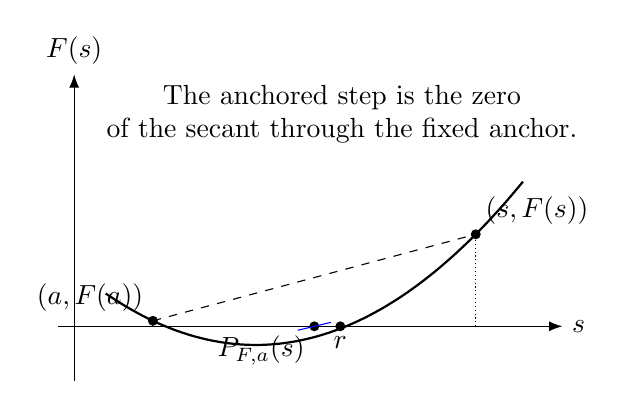
\begin{tikzpicture}[scale=1.0,>=Latex]
    \draw[->] (-0.2,0) -- (6.2,0) node[right] {$s$};
    \draw[->] (0,-0.7) -- (0,3.2) node[above] {$F(s)$};
    \draw[thick,domain=0.4:5.7,smooth,variable=\x] plot ({\x},{0.18*(\x-3)^2+0.25*(\x-3)-0.15});
    \coordinate (r) at (3.38,0);
    \coordinate (a) at (1.0,{0.18*(1.0-3)^2+0.25*(1.0-3)-0.15});
    \coordinate (s) at (5.1,{0.18*(5.1-3)^2+0.25*(5.1-3)-0.15});
    \draw[dashed] (a) -- (s);
    \draw[densely dotted] (1.0,0) -- (a);
    \draw[densely dotted] (5.1,0) -- (s);
    \fill (a) circle (1.8pt) node[above left] {$(a,F(a))$};
    \fill (s) circle (1.8pt) node[above right] {$(s,F(s))$};
    \fill (r) circle (1.8pt) node[below] {$r$};
    \coordinate (p) at (3.05,0);
    \fill (p) circle (1.8pt) node[below left] {$P_{F,a}(s)$};
    \draw[blue] (2.84,-0.05) -- (3.26,0.05);
    \node[align=center] at (3.4,2.7) {The anchored step is the zero\\of the secant through the fixed anchor.};
\end{tikzpicture}
\caption{Anchored Pandrosion as a fixed-anchor secant map.  The root of the secant line is the next iterate $P_{F,a}(s)$.}
\end{figure}

\section{Fixed points and poles}

The fixed-point statement is exact and requires no approximation.

\begin{theorem}[Zeros are fixed points]
Let $F$ be analytic on $U$, let $F(a)\ne0$, and let $r\in U$ be a zero of $F$ with $r\ne a$.  Then
\[
        P_{F,a}(r)=r.
\]
Conversely, if $s\ne a$, $F[a,s]\ne0$, and $P_{F,a}(s)=s$, then $F(s)=0$.
\end{theorem}

\begin{proof}
If $F(r)=0$, then
\[
        F[a,r]=\frac{F(a)}{a-r}.
\]
Therefore
\[
        P_{F,a}(r)=a-\frac{F(a)}{F(a)/(a-r)}=r.
\]
Conversely, suppose $P_{F,a}(s)=s$ and $s\ne a$.  Then
\[
        a-s=\frac{F(a)}{F[a,s]}.
\]
Multiplying by $F[a,s]=(F(a)-F(s))/(a-s)$ gives
\[
        F(a)-F(s)=F(a),
\]
hence $F(s)=0$.
\end{proof}

\begin{remark}[Spurious fixed points]
Under the stated assumptions there are no non-anchor spurious fixed points.  The only obstruction to iteration is not a fake fixed point but a pole, i.e. an equal-value point $F(s)=F(a)$.
\end{remark}

\begin{example}[The monomial poles]
For $F_{p,x}(s)=xs^p-1$ and $a=1$,
\[
        F_{p,x}(s)=F_{p,x}(1)
        \quad\Longleftrightarrow\quad
        xs^p-1=x-1
        \quad\Longleftrightarrow\quad
        s^p=1.
\]
The point $s=1$ is the anchor.  The non-anchor poles are the non-trivial $p$-th roots of unity.  These are exactly the poles visible in the complex monomial map.
\end{example}

\section{Exact multiplier and local residual law}

Let $r$ be a zero of $F$.  The speed of the raw fixed-anchor iteration near $r$ is governed by the derivative of $P_{F,a}$ at $r$.

\begin{theorem}[Exact anchored multiplier]
Let $r$ be a zero of $F$ and assume $F(a)\ne0$, $a\ne r$.  Then $P_{F,a}$ is analytic at $r$ and
\[
        P_{F,a}'(r)=1-\frac{(a-r)F'(r)}{F(a)}.
        \tag{4.1}
\]
Equivalently,
\[
        P_{F,a}'(r)=1-\frac{F'(r)}{F[a,r]}.
        \tag{4.2}
\]
\end{theorem}

\begin{proof}
Put $Q(s)=F[a,s]=(F(a)-F(s))/(a-s)$.  Then
\[
        P_{F,a}(s)=a-\frac{F(a)}{Q(s)},
        \qquad
        P_{F,a}'(s)=F(a)\frac{Q'(s)}{Q(s)^2}.
\]
A direct derivative gives
\[
        Q'(s)=\frac{-F'(s)(a-s)+F(a)-F(s)}{(a-s)^2}.
\]
At $s=r$, $F(r)=0$, so
\[
        Q(r)=\frac{F(a)}{a-r},
        \qquad
        Q'(r)=\frac{F(a)-(a-r)F'(r)}{(a-r)^2}.
\]
Substitution yields
\[
        P_{F,a}'(r)=F(a)\frac{F(a)-(a-r)F'(r)}{(a-r)^2}\frac{(a-r)^2}{F(a)^2}
        =1-\frac{(a-r)F'(r)}{F(a)}.
\]
Since $F[a,r]=F(a)/(a-r)$, (4.2) follows.
\end{proof}

Formula (4.2) is the main residual identity of the paper.  It says that the multiplier is the defect between the tangent slope $F'(r)$ and the secant slope $F[a,r]$ from the anchor to the root.  If the secant slope equals the tangent slope, the linear residual vanishes.

\begin{corollary}[Local attraction criterion]
Let $r$ be a simple zero of $F$.  The fixed point $r$ is locally attracting for the raw anchored iteration whenever
\[
        \left|1-\frac{F'(r)}{F[a,r]}\right|<1.
        \tag{4.3}
\]
It is superattracting for the raw map precisely when $F[a,r]=F'(r)$.
\end{corollary}

\begin{proof}
This is the standard fixed-point criterion applied to the exact multiplier (4.2).
\end{proof}

The condition $F[a,r]=F'(r)$ is automatic for affine functions.  Thus an affine equation is solved in one anchored step, independently of the current state.

\subsection{The anchor-near-root expansion}

The next result is the general version of the monomial logarithmic multiplier law.

\begin{theorem}[Anchor-near-root expansion]
Let $r$ be a simple zero of an analytic function $F$.  Put $\eps=a-r$.  As $a\to r$ with $a\ne r$,
\[
        P_{F,a}'(r)
        =\frac{F''(r)}{2F'(r)}\eps
        +\left(
            \frac{F'''(r)}{6F'(r)}
            -\frac{F''(r)^2}{4F'(r)^2}
        \right)\eps^2
        +O(\eps^3).
        \tag{4.4}
\]
In particular,
\[
        P_{F,a}'(r)=\frac{F''(r)}{2F'(r)}(a-r)+O((a-r)^2).
        \tag{4.5}
\]
\end{theorem}

\begin{proof}
Write
\[
        F(a)=F'(r)\eps+\frac{F''(r)}{2}\eps^2+\frac{F'''(r)}{6}\eps^3+O(\eps^4).
\]
Then
\[
        \frac{\eps F'(r)}{F(a)}
        =\left(
            1+\frac{F''(r)}{2F'(r)}\eps
             +\frac{F'''(r)}{6F'(r)}\eps^2
             +O(\eps^3)
          \right)^{-1}.
\]
Expanding the reciprocal and using (4.1) gives (4.4).
\end{proof}

\begin{corollary}[The monomial local law]
For $F_{p,y}(s)=ys^p-1$, anchor $a=1$, and $y=e^\delta$ with $\delta\to0$, the fixed point is $r=e^{-\delta/p}$ and
\[
        P_{F_{p,y},1}'(r)=\frac{p-1}{2p}\delta+O(\delta^2).
\]
\end{corollary}

\begin{proof}
For $F_{p,y}$,
\[
        \frac{F''(r)}{2F'(r)}=\frac{p-1}{2r}.
\]
Also
\[
        1-r=1-e^{-\delta/p}=\frac{\delta}{p}+O(\delta^2).
\]
Substituting into (4.5) gives the claim.
\end{proof}

\subsection{Two-point local error}

The fixed-anchor map is a secant map with one endpoint held fixed.  Its local error is therefore a product of the anchor error and the current error.

\begin{theorem}[Two-point local error]
Let $r$ be a simple zero of an analytic function $F$.  There are constants $C>0$ and $\rho>0$ such that, whenever
$0<|a-r|<\rho$ and $|s-r|<\rho$,
\[
        P_{F,a}(s)-r
        =\frac{F''(r)}{2F'(r)}(a-r)(s-r)
        +R(a,s),
        \tag{4.6}
\]
with
\[
        |R(a,s)|\le C|a-r|\,|s-r|\,(|a-r|+|s-r|).
        \tag{4.7}
\]
\end{theorem}

\begin{proof}
Set $\alpha=a-r$ and $\sigma=s-r$.  Since $F'(r)\ne0$, write
\[
        F(r+w)=A w+B w^2+O(w^3),
        \qquad A=F'(r),\quad B=\frac{F''(r)}{2}.
\]
The secant slope satisfies
\[
        F[a,s]=A+B(\alpha+\sigma)+O(|\alpha|^2+|\alpha\sigma|+|\sigma|^2).
\]
Using the equivalent secant form
\[
        P_{F,a}(s)=s-\frac{F(s)}{F[a,s]},
\]
we get
\[
\begin{aligned}
        P_{F,a}(s)-r
        &=\sigma-\frac{A\sigma+B\sigma^2+O(\sigma^3)}
        {A+B(\alpha+\sigma)+O(|\alpha|^2+|\alpha\sigma|+|\sigma|^2)}  \\
        &=\frac{B}{A}\alpha\sigma
          +O(|\alpha|\,|\sigma|\,(|\alpha|+|\sigma|)).
\end{aligned}
\]
Since $B/A=F''(r)/(2F'(r))$, the result follows after shrinking $\rho$ if necessary.
\end{proof}

This theorem explains the method's character.  With $a$ fixed, the factor $|a-r|$ is frozen, so the iteration is generally linear.  If the anchor is updated, the error product becomes the classical secant mechanism.

\begin{corollary}[Multiple roots]
If $r$ is a multiple zero of $F$, $F(a)\ne0$, and $a\ne r$, then
\[
        P_{F,a}'(r)=1.
\]
Thus fixed-anchor Pandrosion does not remove the usual difficulty caused by multiple roots.
\end{corollary}

\begin{proof}
At a multiple root $F'(r)=0$.  Formula (4.1) gives $P_{F,a}'(r)=1$.
\end{proof}

\section{Recovery of the monomial scheme}

We now verify that the monomial paper is obtained exactly from the anchored divided-difference construction.

\begin{theorem}[Exact monomial recovery]
Let $p\ge2$, $x\ne0$, and
\[
        F_{p,x}(s)=xs^p-1,
        \qquad a=1.
\]
Then
\[
        F_{p,x}[1,s]=xS_p(s),
        \qquad
        S_p(s)=1+s+\cdots+s^{p-1},
\]
and therefore
\[
        P_{F_{p,x},1}(s)
        =1-\frac{x-1}{xS_p(s)}
        =h_{p,x}(s).
\]
If $x>0$ and $\alpha=x^{1/p}$ is the positive root scale, then at $r=\alpha^{-1}$,
\[
        P_{F_{p,x},1}'(r)=1-\frac{p}{S_p(\alpha)}.
        \tag{5.1}
\]
\end{theorem}

\begin{proof}
The identity
\[
        1-s^p=(1-s)S_p(s)
\]
gives
\[
        F_{p,x}[1,s]
        =\frac{x-1-(xs^p-1)}{1-s}
        =x\frac{1-s^p}{1-s}=xS_p(s).
\]
This proves the map identity.  At $r=\alpha^{-1}$, one has $xr^p=1$ and
\[
        F_{p,x}'(r)=pxr^{p-1}=p\alpha.
\]
Moreover
\[
        F_{p,x}[1,r]=xS_p(r)
        =\alpha^p\sum_{k=0}^{p-1}\alpha^{-k}
        =\alpha S_p(\alpha).
\]
Thus (4.2) gives
\[
        P_{F_{p,x},1}'(r)=1-\frac{p\alpha}{\alpha S_p(\alpha)}=1-\frac{p}{S_p(\alpha)}.
\]
\end{proof}

This theorem is the bridge between the first monomial paper and the present general theory.  The finite sum $S_p$ is not an arbitrary denominator; it is the divided difference $F[1,s]$ for the monomial equation $F(s)=xs^p-1$.

\begin{example}[Quadratic equation]
Let $F(s)=s^2-y$ and choose an anchor $a$ with $a^2\ne y$.  Then
\[
        F[a,s]=a+s,
        \qquad
        P_{F,a}(s)=a-\frac{a^2-y}{a+s}.
\]
At the positive root $r=\sqrt{y}$,
\[
        P_{F,a}'(r)=1-\frac{2r}{a+r}=\frac{a-r}{a+r}.
\]
For $a=1$ this is the $p=2$ monomial multiplier after the corresponding change of target.
\end{example}

\section{Real-line convergence criteria}

The exact multiplier gives a simple real criterion.  Suppose $F$ is real-valued on an interval $I\subset\R$, $r\in I$ is a simple zero, and $a\in I$ is an anchor with $F(a)\ne0$.

By the integral form of the divided difference,
\[
        F[a,r]=\int_0^1 F'\bigl(r+t(a-r)\bigr)\dd t.
        \tag{6.1}
\]
Hence the multiplier is
\[
        \lambda_{F,a}(r)=1-\frac{F'(r)}{\int_0^1 F'(r+t(a-r))\dd t}.
        \tag{6.2}
\]

\begin{proposition}[Real attraction criterion]
Assume $F[a,r]\ne0$.  The root $r$ is locally attracting for the raw anchored iteration if and only if
\[
        \left|1-\frac{F'(r)}{F[a,r]}\right|<1.
\]
If $F'(r)$ and $F[a,r]$ are real with the same sign, this is equivalent to
\[
        0<\frac{F'(r)}{F[a,r]}<2.
        \tag{6.3}
\]
\end{proposition}

\begin{proof}
The first statement is the fixed-point criterion.  If the quotient is real, $|1-q|<1$ is equivalent to $0<q<2$.
\end{proof}

\begin{corollary}[A monotonicity sufficient condition]
Assume $F'>0$ on the interval with endpoints $r$ and $a$.
If $F'$ is monotone along the interval and the average slope $F[a,r]$ satisfies
\[
        F[a,r]>\frac12F'(r),
\]
then $r$ is locally attracting.  In particular, if $F'$ is positive and the anchor is placed on the side where the average slope is at least $F'(r)$, then
\[
        0\le \lambda_{F,a}(r)<1.
\]
\end{corollary}

\begin{proof}
The first assertion is exactly (6.3).  If $F[a,r]\ge F'(r)>0$, then $0<F'(r)/F[a,r]\le1$, so $0\le\lambda_{F,a}(r)<1$, except in the affine case where the multiplier is $0$.
\end{proof}

This criterion is intentionally local.  A real orbit can still leave the interval or hit a pole.  The theorem only says what happens once the iterates remain in a pole-free neighborhood of the root.

\section{Charted anchored Pandrosion}

The monomial paper emphasizes that homothety and the reciprocal chart are not post-processing tricks; they are chart choices made before iteration.  The same principle can be stated for general analytic equations.

Let $G(z)=0$ be an equation on a domain $\Omega\subset\C$.  Let $\phi:V\to\Omega$ be a biholomorphic chart and choose an anchor $a\in V$ with $G(\phi(a))\ne0$.  Define
\[
        F_\phi(s)=G(\phi(s)).
\]
The charted anchored Pandrosion map is
\[
        P_{\phi,a}(s)
        =a-\frac{G(\phi(a))}{F_\phi[a,s]}.
        \tag{7.1}
\]
If $\rho$ is a zero of $G$ and $r=\phi^{-1}(\rho)$, then $r$ is a fixed point of $P_{\phi,a}$.

\begin{theorem}[Charted multiplier]
Let $\rho$ be a simple zero of $G$, let $r=\phi^{-1}(\rho)$, and let $G(\phi(a))\ne0$.  Then
\[
        P_{\phi,a}'(r)
        =1-\frac{(a-r)G'(\rho)\phi'(r)}{G(\phi(a))}.
        \tag{7.2}
\]
Moreover, as $a\to r$ in the chart,
\[
        P_{\phi,a}'(r)
        =\frac{1}{2}
        \left(
            \frac{G''(\rho)\phi'(r)}{G'(\rho)}
            +\frac{\phi''(r)}{\phi'(r)}
        \right)(a-r)
        +O((a-r)^2).
        \tag{7.3}
\]
\end{theorem}

\begin{proof}
Apply Theorem 4.1 to $F_\phi=G\circ\phi$.  Since
\[
        F_\phi'(r)=G'(\rho)\phi'(r),
\]
we get (7.2).  Also
\[
        \frac{F_\phi''(r)}{F_\phi'(r)}
        =\frac{G''(\rho)(\phi'(r))^2+G'(\rho)\phi''(r)}{G'(\rho)\phi'(r)}
        =\frac{G''(\rho)\phi'(r)}{G'(\rho)}+\frac{\phi''(r)}{\phi'(r)}.
\]
Then (7.3) follows from (4.5).
\end{proof}

Equation (7.3) is the chart-selection law.  A good chart places the root coordinate $r$ near the anchor $a$ and avoids introducing excessive chart curvature $\phi''/\phi'$.

\begin{example}[Affine and reciprocal chart families]
Fix the coordinate anchor $a=1$.
The affine family
\[
        \phi_B(s)=Bs,
        \qquad B\ne0,
\]
places the anchor at $B$ in the original variable.  A zero $\rho$ is represented by $r=\rho/B$, so choosing $B\approx\rho$ makes $r\approx1$.
The reciprocal family
\[
        \psi_B(s)=\frac{1}{Bs},
        \qquad B\ne0,
\]
places the anchor at $1/B$ and represents $\rho$ by $r=1/(B\rho)$.  This is useful when the natural affine scale is near zero or infinity.  These are the general analytic analogues of direct and reciprocal chart scaling in the monomial setting.
\end{example}

\begin{remark}[What scaling changes]
A pure rescaling of coordinates around a fixed anchor image does not change the local multiplier.  What matters is the image of the anchor under the chart.  In the affine family $\phi_B(s)=Bs$ with coordinate anchor $1$, changing $B$ moves the anchor image from $1$ to $B$.  This is why scaling can change the multiplier.
\end{remark}

\section{Anchor palettes and local covering}

A single anchor may be poorly placed for some roots.  A finite anchor palette is a finite set
\[
        \mathcal{A}=\{a_1,\ldots,a_N\}\subset U
\]
with $F(a_j)\ne0$.  Each anchor defines a map $P_{F,a_j}$.  Near a simple root $r$, the best local anchor is the one with the smallest multiplier
\[
        \min_{a_j\in\mathcal{A}}
        \left|1-\frac{F'(r)}{F[a_j,r]}\right|.
        \tag{8.1}
\]
Since $r$ is not known exactly before solving, (8.1) is a theoretical selection rule.  The next theorem gives a simple covering principle.

\begin{theorem}[Local anchor covering]
Let $K\subset U$ be compact, and suppose every zero of $F$ in $K$ is simple.  Assume there is a compact neighborhood $K_1\Subset U$ of those zeros on which
\[
        |F'(z)|\ge m>0,
        \qquad
        |F''(z)|\le M.
\]
Then there exist constants $h_0>0$ and $C>0$ such that if $r\in K$ is a zero of $F$ and $a\in K_1$ satisfies
\[
        0<|a-r|\le h_0,
\]
then
\[
        |P_{F,a}'(r)|\le C|a-r|.
        \tag{8.2}
\]
Consequently, a palette whose mesh near every zero is at most $h$ has worst local raw multiplier $O(h)$ as $h\to0$.
\end{theorem}

\begin{proof}
By (4.5), for each simple zero $r$,
\[
        P_{F,a}'(r)=\frac{F''(r)}{2F'(r)}(a-r)+O((a-r)^2).
\]
The constants in this expansion are uniform over the finitely many zeros in $K$ because the zeros are simple and $K_1$ is compact.  Taking $h_0$ small enough gives (8.2).
\end{proof}

This result is the general local counterpart of the scale-palette theorem in the monomial paper.  In the monomial case, the special logarithmic structure gives a sharp global minimax statement.  For a general analytic function, the corresponding statement is necessarily local unless additional global geometry is assumed.

\section{Steffensen acceleration}

The raw anchored map is generally only linearly convergent.  Aitken--Steffensen acceleration converts a fixed-point map into a derivative-free higher-order map by evaluating the same fixed-point map twice.

For $P=P_{F,a}$ define
\[
        \Sigma_{F,a}(s)
        =s-\frac{(P(s)-s)^2}{P(P(s))-2P(s)+s},
        \tag{9.1}
\]
where the denominator is nonzero; at a removable singularity, use the analytic continuation.

\begin{theorem}[Quadratic Steffensen--Pandrosion]
Let $r$ be a simple zero of $F$.  Assume $P=P_{F,a}$ is analytic near $r$ and
\[
        \lambda=P'(r)\ne1.
\]
Then $\Sigma_{F,a}$ has a removable singularity at $r$, fixes $r$, and satisfies
\[
        \Sigma_{F,a}(s)-r
        =\frac{\lambda P''(r)}{2(\lambda-1)}(s-r)^2
        +O((s-r)^3).
        \tag{9.2}
\]
In particular, the accelerated map is at least quadratically convergent near $r$.
\end{theorem}

\begin{proof}
Write $e=s-r$ and expand
\[
        P(r+e)=r+\lambda e+c e^2+d e^3+O(e^4),
        \qquad c=\frac12P''(r).
\]
Then
\[
        P(s)-s=(\lambda-1)e+c e^2+d e^3+O(e^4),
\]
and a second substitution gives
\[
        P(P(r+e))=r+\lambda^2e+c\lambda(1+\lambda)e^2+O(e^3).
\]
Therefore
\[
        P(P(s))-2P(s)+s=(\lambda-1)^2e+c(\lambda-1)(\lambda+2)e^2+O(e^3).
\]
Since $\lambda\ne1$, the quotient in (9.1) has a removable singularity at $e=0$.  Dividing the two series yields
\[
        \frac{(P(s)-s)^2}{P(P(s))-2P(s)+s}
        =e-\frac{c\lambda}{\lambda-1}e^2+O(e^3).
\]
Substitution into (9.1) gives
\[
        \Sigma_{F,a}(s)-r=\frac{c\lambda}{\lambda-1}e^2+O(e^3)
        =\frac{\lambda P''(r)}{2(\lambda-1)}e^2+O(e^3).
\]
\end{proof}

\begin{remark}[Derivative-free status]
The map $P_{F,a}$ uses values of $F$ and the fixed value $F(a)$.  The Steffensen map uses $P(s)$ and $P(P(s))$, hence additional values of $F$, but no derivative values.  If one initializes at $s=a$ by using $P(a)=a-F(a)/F'(a)$, then that particular start uses a derivative.  A derivative-free start instead takes any calibration point $b\ne a$ and starts from $P_{F,a}(b)$.
\end{remark}

The condition $\lambda\ne1$ excludes multiple roots, as expected from Corollary 4.7.  If $\lambda=0$, then the displayed quadratic coefficient vanishes and the order is at least quadratic, often higher.

\section{Complex local theory}

The complex theory is naturally meromorphic.  Poles are equal-value points $F(s)=F(a)$, and fixed points are roots of $F$.  The following theorem is the local complex analogue of the real contraction statements.

\begin{theorem}[Seeded complex convergence]
Let $F$ be analytic on a domain $U\subset\C$, let $r\in U$ be a simple zero, and let $a\in U$ satisfy $F(a)\ne0$ and $a\ne r$.  Let
\[
        \lambda=P_{F,a}'(r).
\]
Then there exists $\rho>0$ such that $P_{F,a}$ is analytic on $D(r,\rho)$.
If $|\lambda|<1$, then after shrinking $\rho$ if necessary, $P_{F,a}$ maps $D(r,\rho)$ into itself and every orbit starting in $D(r,\rho)$ converges to $r$.
If $\lambda\ne1$, the Steffensen map $\Sigma_{F,a}$ is analytic on a possibly smaller disk after filling its removable singularity at $r$, and there is a constant $C_r$ such that
\[
        |\Sigma_{F,a}(s)-r|\le C_r|s-r|^2
        \qquad (s\in D(r,\rho)).
\]
\end{theorem}

\begin{proof}
Since $F(a)\ne0$ and $F(r)=0$, the denominator $F[a,r]=F(a)/(a-r)$ is nonzero.  Hence $P_{F,a}$ is analytic in some disk around $r$ avoiding the pole set.  The raw convergence statement follows from the standard contraction theorem applied on a sufficiently small disk when $|\lambda|<1$.  The Steffensen statement follows from Theorem 9.1 and the maximum principle on a small pole-free circle around $r$.
\end{proof}

A practical complex implementation would use an anchor selector.  Given a finite set of candidate anchors or charted anchors, assign an initial point to the anchor with the smallest estimated residual factor or smallest chart distance to the suspected root.  For monomials the anchors and poles have cyclotomic structure; for a general analytic function they are determined by the zeros and equal-value sets of $F$.

\section{Relation with Newton and the secant method}

Anchored Pandrosion sits between three familiar ideas.

First, if the current point equals the anchor and $F'(a)\ne0$, then
\[
        P_{F,a}(a)=a-\frac{F(a)}{F'(a)},
\]
which is Newton's correction at the anchor.  This is a limiting value of the anchored map, not the rule used at every step.

Second, if the anchor is updated by using the previous iterate, then anchored Pandrosion becomes the classical secant method:
\[
        s_{n+1}=P_{F,s_{n-1}}(s_n).
\]
The superlinear behavior of the secant method is reflected in the two-point product law (4.6).

Third, if the anchor is kept fixed, the method becomes a linearly convergent fixed-point iteration with exact multiplier (4.1).  Steffensen acceleration then cancels that linear term without requiring derivatives.

Thus the originality claim is intentionally limited.  The fixed-anchor secant formula is classical.  The contribution of this paper is to identify it as the general analytic form of monomial Pandrosion and to organize its residual behavior through anchors and charts.  This also prevents an overstatement: for ordinary scalar root finding, Newton, Halley, and well-designed multipoint methods are usually more efficient in work-normalized terms.  Anchored Pandrosion is valuable when the goal is an explicit derivative-free fixed-point operator whose multiplier can be read from a divided difference and improved by anchor or chart placement.

\section{Numerical illustrations}

The following small experiments are included only to check the local theory.  They are not speed claims.  Raw anchored Pandrosion uses
\[
        s_{n+1}=P_{F,a}(s_n),
\]
Steffensen--Pandrosion uses (9.1), and Newton uses $s_{n+1}=s_n-F(s_n)/F'(s_n)$ as a standard derivative-based baseline.  The stopping condition is
\[
        |s_n-r|\le 10^{-12}\max(1,|r|).
\]

\begin{center}
\begin{tabular}{@{}llcccccc@{}}
\toprule
Equation & root $r$ & anchor $a$ & start $s_0$ & $|\lambda|$ & raw & Steff. & Newton \\
\midrule
$e^s-2=0$      & $0.693147$ & $1.0$ & $0.50$ & $0.145592$ & $14$ & $3$ & $4$ \\
$\cos s-1/2=0$ & $1.047198$ & $1.0$ & $1.25$ & $0.014192$ & $7$  & $2$ & $4$ \\
$s^3+s-2=0$   & $1.000000$ & $1.2$ & $0.40$ & $0.137931$ & $14$ & $3$ & $6$ \\
$s^3+s-2=0$   & $1.000000$ & $0.8$ & $1.30$ & $0.162791$ & $15$ & $3$ & $5$ \\
\bottomrule
\end{tabular}
\end{center}

The table shows the predicted behavior: smaller $|\lambda|$ gives shorter raw fixed-point convergence, and Steffensen acceleration collapses the linear regime to a few quadratic steps.  Newton remains a strong baseline; the role of Pandrosion here is not to replace Newton, but to expose how the fixed anchor controls the residual multiplier.

The cubic example also illustrates anchor placement.  For $F(s)=s^3+s-2$, the root is $r=1$.  If one chooses the distant anchor $a=0$, then
\[
        F(a)=-2,
        \qquad F'(r)=4,
        \qquad \lambda=1-\frac{(0-1)4}{-2}=-1,
\]
which is neutral in the linearized sense.  Moving the anchor to $a=1.2$ changes the multiplier to $0.137931\ldots$, producing a genuine local contraction.

\section{Conclusion}

The monomial Pandrosion denominator $S_p$ is a divided difference in disguise.  Replacing it by $F[a,s]$ gives a general anchored fixed-point scheme
\[
        P_{F,a}(s)=a-\frac{F(a)}{F[a,s]}.
\]
The scheme has three basic structural facts:
\begin{enumerate}[label=\textup{(\roman*)},leftmargin=*]
\item roots of $F$ are exactly the non-anchor fixed points of the map;
\item poles are exactly equal-value points $F(s)=F(a)$;
\item the local residual multiplier is
\[
        1-\frac{F'(r)}{F[a,r]}.
\]
\end{enumerate}

The anchor-near-root expansion
\[
        P_{F,a}'(r)=\frac{F''(r)}{2F'(r)}(a-r)+O((a-r)^2)
\]
is the general version of the monomial logarithmic law.  It gives the chart-selection principle: choose an anchor or chart in which the transformed root lies close to the fixed anchor and away from the equal-value poles.  The two-point error law
\[
        P_{F,a}(s)-r\sim \frac{F''(r)}{2F'(r)}(a-r)(s-r)
\]
explains why a fixed anchor gives linear convergence but a moving anchor recovers secant behavior.  Finally, Steffensen acceleration preserves the derivative-free character of the fixed-point map while giving local quadratic convergence.

This paper therefore supplies the natural sequel to the monomial theory: Pandrosion is not tied to $s^p$.  The monomial case is the exact geometric-sum model of a broader anchored divided-difference fixed-point framework.

\section*{Acknowledgments}
The author thanks the earlier monomial Pandrosion manuscript for the motivating residual profile, chart-scaling principle, and Steffensen comparison.  This draft was prepared as a mathematical continuation of that work; the author remains responsible for verification, revision, and submission decisions.

\begin{thebibliography}{99}

\bibitem{BesevicMonomial2026}
I. Besevic,
\emph{A Monomial Pandrosion Scheme: Contraction, Chart Scaling, and Steffensen Acceleration for $z^p=x$},
Independent Mathematical Research, manuscript, May 2026.

\bibitem{Aitken1926}
A. C. Aitken,
``On Bernoulli's numerical solution of algebraic equations,''
\emph{Proceedings of the Royal Society of Edinburgh} \textbf{46} (1926), 289--305.

\bibitem{Steffensen1933}
J. F. Steffensen,
``Remarks on iteration,''
\emph{Skandinavisk Aktuarietidskrift} \textbf{16} (1933), 64--72.

\bibitem{Ostrowski1966}
A. M. Ostrowski,
\emph{Solution of Equations and Systems of Equations},
2nd ed., Academic Press, 1966.

\bibitem{Traub1964}
J. F. Traub,
\emph{Iterative Methods for the Solution of Equations},
Prentice-Hall, 1964.

\bibitem{Householder1970}
A. S. Householder,
\emph{The Numerical Treatment of a Single Nonlinear Equation},
McGraw-Hill, 1970.

\bibitem{OrtegaRheinboldt1970}
J. M. Ortega and W. C. Rheinboldt,
\emph{Iterative Solution of Nonlinear Equations in Several Variables},
Academic Press, 1970.

\bibitem{Henrici1974}
P. Henrici,
\emph{Applied and Computational Complex Analysis},
Wiley, 1974--1986.

\bibitem{Milnor2006}
J. Milnor,
\emph{Dynamics in One Complex Variable},
3rd ed., Princeton University Press, 2006.

\bibitem{Petkovic2013}
M. S. Petkovic, B. Neta, L. D. Petkovic, and J. Dzunic,
\emph{Multipoint Methods for Solving Nonlinear Equations},
Academic Press, 2013.

\end{thebibliography}

\end{document}
